\chapter{Ensayos y Resultados}
\label{Chapter4}

% \section{Infraestructura para el Desarrollo}

\section{Simulación y Verificación}

La verificación y validación de código y modelos por medio de simulación es
un aspecto crucial para garantizar calidad y reducir tiempos de desarrollo,
sobre todo en sistemas críticos. La verificación garantiza con simulaciones y
permite la corrección del código, antes de hacer pruebas en el mundo real, que
son más lentas y costosas. La validación se relaciona con la conexión del
desarrollo con el mundo real y su uso previsto, implica contar con el
\textit{hardware} y el instrumental de medición. Además, en sistemas de alta
complejidad la simulación permite probar cada módulo por separado, técnica que
facilita la integración y permite distinguir con claridad los errores, lo que
acelera proceso de aprendizaje y comprensión del sistema. Por otro lado al ser
capaces de simular datos de cierto modelo, se garantiza que uno entiende el
modelo, sus restricciones y limitaciones.

% En este trabajo se llevaron a cabo test unitarios para cada módulo básico del
% desarrollo e incluso aquellos que integraban varios submódulos, usando GHDL,
% cocotb e integración continua en Github, pero para la verificación del sistema
% completo fue necesario usar Quartus y ModelSim, ya que no se contaba con los
% modelos de los Transceivers debido a que son herramientas propietarias.

\subsection{\textit{cocotb}}
\textit{cocotb} (por sus siglas en inglés \textit{COroutine based COsimulation
TestBench}) es un entorno de \textit{TestBench} de verificación de simulación
basado en corrutinas para verificar RTL (por sus siglas en inglés
\textit{Register Transfer Level}) descriptos en VHDL y SystemVerilog utilizando
Python.

Este \textit{Framework} es completamente gratuito, de código abierto (Licencia
BSD) y alojado en GitHub.\textit{cocotb} requiere un simulador para simular el
diseño HDL (por sus siglas en inglés \textit{Hardware Description Language}) y
se puede utilizar con una variedad de simuladores en multiples sistemas
operativos.

\textit{cocotb} fomenta la filosofía de reutilización de diseño y pruebas
aleatorias que UVM, sin embargo, está implementado en Python.

Con \textit{cocotb}, los HDL tradicionales se utilizan solo para el diseño en
sí, no para el banco de pruebas. Además, tiene soporte incorporado para
integrarse con sistemas de integración continua y fue diseñado específicamente
para reducir la sobrecarga de la creación de una prueba.También descubre
automáticamente las pruebas, por lo que no se requiere un paso adicional para
agregar una prueba a una regresión.

La verificación se realiza integramente con Python, lo cual tiene varias
ventajas por sobre el uso de SystemVerilog o VHDL para la verificación:

\begin{itemize}
  \item Es rápido escribir en Python, es un lenguaje muy productivo.
  \item Es fácil interfacear con otros lenguajes.
  \item Python tiene una enorme biblioteca de código existente para reutilizar.
  \item Python es interpretado: las pruebas se pueden editar y volver a ejecutar
  sin tener que recompilar el diseño.
  \item Python es popular: muchos más desarrolladores conocen Python que
  VHDL o SystemVerilog.
\end{itemize}

\subsection{Funcionamiento de \textit{cocotb}}

Un banco de pruebas típico de \textit{cocotb} no requiere código RTL adicional.
El Diseño Bajo Prueba (DUT, por sus siglas en inglés \textit{Design-Device
under Test}) se instancía como el \textit{toplevel} en el simulador sin ningún
código que haga de interfaz o \textit{wrapper}.\textit{cocotb} proporciona
estímulos a las entradas del DUT (o incluso más abajo en la jerarquía) y
supervisa las salidas directamente desde Python.

\begin{figure}[h]
  \centering
  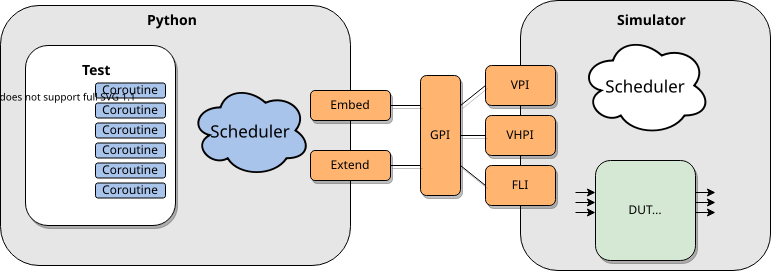
\includegraphics[width=0.7\textwidth]{./Figures/cocotb_overview.png}
  \caption{Visión general de \textit{cocotb}.}
\end{figure}

% Una prueba es simplemente una función Python. En cualquier momento, el simulador
% está avanzando en el tiempo o el código Python se está ejecutando. La palabra
% clave \texttt{await} se utiliza para indicar cuándo pasar el control de
% ejecución de vuelta al simulador. Una prueba puede generar múltiples corutinas,
% lo que permite flujos de ejecución independientes.

\subsection{Estructura Genérica de los \textit{Test} y sus resultados}

\section{Integración Continua}

La integración continua (CI, del inglés \textit{continuous integration}) es una
práctica que nace de la ingeniería de software, pero que en los últimos años se
a ido extendiendo a otras ramas de la ingeniería, que consiste en hacer
integraciones automáticas de un proyecto con cierta regularidad para así poder
detectar errores cuanto antes. Se entiende por integración la compilación o
síntesis y ejecución de pruebas de un proyecto completo y sus subsistemas. 

Por lo general se necesita un sistema de control de versiones que acompañe y
ejecute del proceso de CI\@. Los mismos también se complementan con otras
comprobaciones como las pruebas automatizadas de calidad del código, las
herramientas de revisión de estilo de sintaxis, entre otras.

Para pasar en limpio, los beneficios comúnmente citados de la integración
continua incluyen:
\begin{itemize}
  \item Detección temprana y mejorada de errores, y métricas que le permiten
  abordar los errores a tiempo, a veces tras solo unos minutos de la incorporación.
  \item Progreso continuo y demostrado para mejorar la retroalimentación.
  \item Mejor colaboración en equipo: todos los miembros del equipo pueden.
  cambiar el código, integrar el sistema y determinar rápidamente los conflictos
  con otras partes del del mismo.
  \item Integración mejorada del sistema, lo que reduce las sorpresas al final
  del ciclo de vida del desarrollo.
  \item Menos cambios paralelos para la fusión y prueba.
  \item Reducción de cantidad de errores durante las pruebas del sistema.
  \item Sistemas actualizados constantemente en los que realizar las pruebas.
\end{itemize}

En el caso de este trabajo se optó por usar Git como sistema de control de
versiones, más específicamente Github, que con Github Actions también entrega
la funcionalidad de integración continua.

% \section{Quartus y ModelSim}

\section{Resultados}

\subsection{Resultados Generales}

\subsection{Resultados por módulo}
